\documentclass{article}
\usepackage{amsmath,mathtools}
\usepackage{amssymb}
\usepackage[dvipsnames]{xcolor}
\usepackage{graphicx}
\usepackage{tikz}
\usepackage{float}
\usepackage{subcaption}
\usepackage{pgfplots}
\usetikzlibrary{arrows}
\usetikzlibrary{datavisualization.formats.functions}
\usepgfplotslibrary{fillbetween}
\usetikzlibrary{patterns}
\usepackage{xargs}
\usepackage{enumitem}
\usepackage{systeme}
\usepackage{centernot}
\usepackage{physics}
\usepackage{xfrac}
\usepackage{titling}
\usepackage{forest}
\usepackage[margin=1in]{geometry}
\usepackage[skins,theorems]{tcolorbox}
\tcbset{highlight math style={enhanced,
  colframe=blue,colback=white,arc=0pt,boxrule=1pt}}

% calculus commands
\renewcommand{\eval}[3]{\left[#1\right]_{#2}^{#3}}

% linear algebra commands
\newcommand{\icol}[1]{% inline column vector
  \begin{bsmallmatrix}#1\end{bsmallmatrix}%
}
\renewcommand\vec{\mathbf}
\newenvironment{sysmatrix}[1]
{\left[\begin{array}{@{}#1@{}}}
{\end{array}\right]}
\newcommand{\ro}[1]{%
\xrightarrow{\mathmakebox[\rowidth]{#1}}%
}
\newlength{\rowidth}% row operation width
\AtBeginDocument{\setlength{\rowidth}{3em}}

%set theory commands
\newcommand{\pset}[1]{\mathcal P(#1)}
\newcommand{\card}[1]{\operatorname{card}(#1)}
\newcommand{\R}{\mathbb R}
\newcommand{\N}{\mathbb N}
\newcommand{\Z}{\mathbb Z}

%optimization commands
\DeclareMathOperator*{\argmax}{arg\,max}
\DeclareMathOperator*{\argmin}{arg\,min}

%misc commands
\newcommand*\circled[1]{\tikz[baseline=(char.base)]{
             \node[shape=circle,draw,inner sep=2pt] (char) {#1};}}

\setlength{\droptitle}{-7em}   % This is your set screw

\begin{document}

\title{Linear Optimization\\HW \#12}
\author{Ozaner Hansha}
\date{April 27, 2021}
\maketitle

\subsection*{Problem 11.5.2}
\noindent\textbf{Problem:} Explicitly give an example of a Traveling Salesman Problem (other than ones in this chapter!) where there is no solution.
\bigskip

\noindent\textbf{Solution:} Consider a TSP with three cities $\mathcal C=\{1,2,3\}$ and where no city is accessible from any other:
$$S_1=S_2=S_2=\emptyset$$

Clearly then, the TSP has no solution as given any starting point $j$, it is impossible to reach any other city, much less all of them, in a finite amount of time.

\subsection*{Problem 11.5.4}
\noindent\textbf{Problem:} Assume that every city is accessible from every other city. Show there is a valid route that satisfies the constraints.
\bigskip

\noindent\textbf{Solution:} Given a TSP with $n$ cities where for each $j$ we have that:
$$S_j=[1..n]$$

There is always a solution. Namely, starting at city $j$, at time $t$ the following step is made: travel to city $j+t \mod n$. After $n-1$ time steps, every city will have been visited.

\subsection*{Problem 11.5.6}
\noindent\textbf{Problem:} Choose a collection of cities, a starting city, and distances between them so that the greedy algorithm does not give a route of minimal distance.
\bigskip

\noindent\textbf{Solution:} Consider a TSP with 5 cities and the given connections:
\begin{center}
  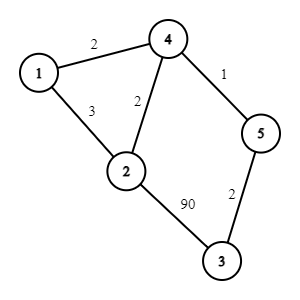
\includegraphics[scale=.5]{graph.png}
\end{center}
Starting at city 1, the greedy algorithm would give the following path:
$$\underbrace{1\to4\to5\to3\to2}_{2+1+2+90=95}$$

We can show this is not a route of minimal distance by demonstrating a shorter route:
$$\underbrace{1\to2\to4\to5\to3}_{3+2+1+2=8}$$

\subsection*{Problem 11.5.8}
\noindent\textbf{Problem:} Without doing out the algebra, find upper and lower bounds for the sum approximating the Insertion Algorithm’s run-time:
$$\sum^n_{k=1}k(n-(k-1))$$ 

How close can you get to the true value?
\bigskip

\noindent\textbf{Solution:} Note the following:
$$\sum^n_{k=1}k(n-(k-1))=\sum^n_{k=1}kn-\sum^n_{k=1}k^2+\sum^n_{k=1}k$$

And so an upper bound on this run time is given by:
\begin{align*}
  \sum^n_{k=1}kn+\sum^n_{k=1}k&=(n+1)\sum^n_{k=1}k\\
  &=(n+1)\frac{n(n+1)}{2}\\
  &=\frac{n(n+1)^2}{2}
\end{align*}

A lower bound is of course 0. Note sure if you wanted something more clever, while not doing algebra...

There is a closed form for the true value since we can express the sum of squares from 1 to $n$ as a closed expression just as we did the sum of integers. So we can get arbitrarily close to this approximation formula.

\subsection*{Problem 11.5.11}
\noindent\textbf{Problem:} Choose a collection of cities, a starting city, and distances between them so that the insertion algorithm does not give a route of minimal distance.
\bigskip

\noindent\textbf{Solution:} Consider a TSP with 5 cities and the given connections:
\begin{center}
  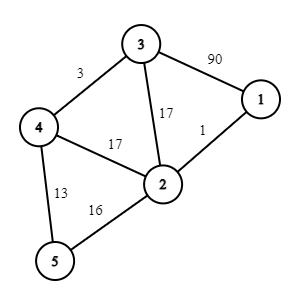
\includegraphics[scale=.5]{graph2.png}
\end{center}

Starting at city 1, the insertion path algorithm (that is, adding new cities in the most locally optimal way, in order) gives:
$$\underbrace{1\to2\to3\to4\to5}_{1+17+3+13=34}$$

We can show that this s not optimal by demonstrating a shorter path:
$$\underbrace{1\to2\to5\to4\to3}_{1+16+13+3=33}$$

\subsection*{Problem 11.5.13}
\noindent\textbf{Problem:} Choose a collection of cities, a starting city, and distances between them so that the sub-problem method does not give a route of minimal distance.
\bigskip

\noindent\textbf{Solution:} For an example with group size greater than 1, consider the following:
\begin{center}
  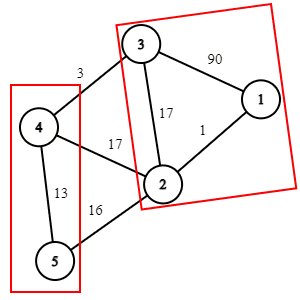
\includegraphics[scale=.5]{graph3.png}
\end{center}

Here the optimal path for the subgroups are:
$$\underbrace{1\to2\to3}_{1+17=18}\qquad\underbrace{4\to5}_{13}$$

And, assuming our strategy is to connect them with the smallest edge possible (i.e. connect them using $(3,4)$), the total path length is:
$$\underbrace{\underbrace{1\to2\to3}_{1+17=18}\underbrace{\to}_{3}\underbrace{4\to5}_{13}}_{18+3+13=34}$$

Notice that this is the same example used in problem 11, which we have already shown to have a shorter path given by:
$$\underbrace{1\to2\to5\to4\to3}_{1+16+13+3=33}$$

And so, the sub-divide method need not provide an optimal route.

\subsection*{Problem 13.7.1}
\noindent\textbf{Problem:} Find all fixed points for the function $f:[0,1]\to[0,1]$ given by:
$$f(x)=x(1-x)$$
\bigskip

\noindent\textbf{Solution:} This is the same as finding the solutions to:
\begin{align*}
  f(x)&=x\\
  x(1-x)&=x\\
  1-x&=1\tag{$x=0$ is a solution}\\
  0&=x\\
\end{align*}

And so the only fixed point of $f(x)$ is at $x=0$.

\subsection*{Problem 13.7.2}
\noindent\textbf{Problem:} Find all fixed points for the function $f:[0,1]^2\to[0,1]^2$ given by:
$$f(x,y)=\left(xy,\frac{x^2+y^2}{2}\right)$$
\bigskip

\noindent\textbf{Solution:} First we will find the conditions for which the $x$ component is equal to $x$:
\begin{align*}
  xy&=x\\
  y&=1\tag{$x=0$ is a solution}
\end{align*}

Now, keeping $x=0$ we will find when the $y$ component is $y$:
\begin{align*}
  f(0,y)&=y\\
  \frac{y^2}{2}&=y\\
  y^2&=2y\\
  y&=2\tag{$y=0$ is a solution}
\end{align*}

And so our first set of fixed points are: $(0,2), (0,0)$. Next we will do the same with $y=1$:
\begin{align*}
  f(x,1)&=1\\
  \frac{x^2+1}{2}&=1\\
  x^2+1&=2\\
  x^2&=1\\
  x&=\pm1
\end{align*}

And so our second set of fixed points are: $(1,1), (-1,1)$. In total, this function has 4 real fixed points given by:
$$(0,2), (0,0), (1,1), (-1,1)$$

\end{document}